\documentclass[a4paper,fleqn]{cas-dc}

\usepackage[numbers]{natbib}
\usepackage[utf8]{inputenc}
\usepackage[T1]{fontenc}
\usepackage{amsmath,amssymb}
\usepackage{graphicx}
\usepackage{booktabs}
\usepackage{multirow}
\usepackage{xcolor}
\usepackage{tikz}
\usetikzlibrary{arrows.meta,positioning,calc,decorations.pathreplacing}
\usepackage{microtype}
\usepackage{subcaption}

\begin{document}
\let\WriteBookmarks\relax
\def\floatpagepagefraction{1}
\def\textpagefraction{.001}

\shorttitle{Evaluating Stream Mapping Strategies for MQTT over QUIC}
\shortauthors{F. Bracht}

\title[mode=title]{Evaluating Stream Mapping Strategies for MQTT over QUIC}

\author[1]{Fabricio Bracht}
\cormark[1]
\ead{fabracht@gmail.com}

\credit{Conceptualization, Methodology, Software, Investigation, Data curation, Writing -- original draft, Writing -- review \& editing, Visualization}

\affiliation[1]{organization={Independent Researcher},
            country={}}

\cortext[1]{Corresponding author}

\begin{abstract}
MQTT, the dominant IoT messaging protocol, operates over TCP, where head-of-line (HOL) blocking couples logically independent topic flows: a single packet loss delays delivery across all topics sharing a connection. We define three configurable stream mapping strategies---control-only, per-topic, and per-publish---for running MQTT over QUIC, each offering a different point in the isolation--overhead tradeoff space. We implement these strategies in \texttt{mqtt5}, an open-source MQTT library, and evaluate across five experiments on GCP infrastructure under controlled network impairment. Using inter-topic latency spread and spike isolation ratio to quantify HOL blocking, we find that per-topic QUIC provides meaningful topic-level isolation under loss: spread amplifies 200$\times$ at 5\% packet loss versus 1.2$\times$ for TCP, and 27\% of latency spikes affect individual topics independently versus less than 2\% for TCP. TCP outperforms QUIC in throughput at 0\% loss, but under loss ($\geq$1\%) QUIC outperforms TCP by up to 2.8$\times$ while providing encryption by default. We additionally evaluate QUIC datagram transport, finding no statistically significant performance difference from stream transport at representative IoT RTTs. These results provide concrete strategy selection guidelines for deploying MQTT over QUIC in IoT environments.
\end{abstract}

\begin{highlights}
\item Three stream mapping strategies for MQTT over QUIC evaluated
\item Per-topic QUIC amplifies inter-topic spread 200$\times$ under 5\% loss
\item QUIC outperforms TCP in throughput under loss by up to 2.8$\times$
\item Frame packing policy interacts asymmetrically with stream lifetime
\item QUIC datagrams show no significant advantage over stream transport
\end{highlights}

\begin{keywords}
MQTT \sep QUIC \sep IoT \sep head-of-line blocking \sep stream multiplexing
\end{keywords}

\maketitle

%% --- Introduction ---

\section{Introduction}
\label{sec:introduction}

MQTT is the dominant messaging protocol for Internet of Things (IoT) deployments, widely adopted for device-to-cloud communication across industrial, smart city, and consumer IoT platforms~\cite{mishra2020mqtt-survey}. MQTT's publish-subscribe model, lightweight framing, and multiple quality-of-service levels make it well-suited for constrained devices and unreliable networks~\cite{mqtt-v5-spec}.

However, MQTT operates over TCP, which introduces a fundamental limitation: \emph{head-of-line (HOL) blocking}. When an IoT device publishes to multiple topics over a single TCP connection---as is common for devices reporting temperature, humidity, GPS, and status simultaneously---a packet loss on any one topic's data blocks delivery of \emph{all} topics until retransmission completes. This creates artificial coupling between logically independent data flows, increasing tail latency and reducing the responsiveness of multi-topic workloads.

QUIC~\cite{rfc9000}, the transport protocol underlying HTTP/3, addresses HOL blocking through \emph{stream multiplexing}: multiple independent streams share a single connection, each with its own flow control and loss recovery. A lost packet on one stream does not block data on other streams. This property has been extensively studied for web traffic~\cite{langley2017quic, kakhki2017quic, marx2020hol, yu2021quic}, but its application to IoT messaging protocols remains largely unexplored.

Running MQTT over QUIC is not simply a matter of replacing the TCP socket. The question of \emph{how} to map MQTT's control and data packets onto QUIC streams admits multiple answers, each with different performance characteristics. A single-stream approach (equivalent to TCP) gains QUIC's security and connection management benefits but not HOL blocking elimination. A per-topic approach maps each MQTT topic to a dedicated QUIC stream, providing topic-level isolation. A per-message approach creates a new stream for each PUBLISH, maximizing isolation at the cost of stream management overhead.

In this paper, we define three configurable stream mapping strategies for MQTT over QUIC, implement them in \texttt{mqtt5}, an open-source MQTT library, and evaluate them across five experiments on GCP infrastructure under controlled network impairment.

Our contributions are:
\begin{enumerate}
\item Three stream mapping strategies (control-only, per-topic, per-publish) for MQTT over QUIC with a lightweight flow header protocol for stream demultiplexing.
\item The first empirical evaluation of MQTT stream mapping strategies under controlled network impairment, quantifying HOL blocking and throughput.
\item An evaluation of QUIC datagram transport for MQTT as an alternative to stream-based delivery.
\item An open-source implementation with integrated benchmarking tools.
\end{enumerate}

The remainder of this paper is organized as follows. Section~\ref{sec:background} covers MQTT, QUIC, and related work. Section~\ref{sec:architecture} describes the stream mapping architecture. Section~\ref{sec:implementation} details the implementation. Section~\ref{sec:evaluation} presents experimental results. Section~\ref{sec:discussion} discusses strategy selection guidelines and future directions. Section~\ref{sec:conclusion} concludes.

%% --- Background and Related Work ---

\section{Background and Related Work}
\label{sec:background}

\subsection{MQTT Protocol}

MQTT~\cite{mqtt-v5-spec} provides three quality-of-service levels (QoS~0: at-most-once, QoS~1: at-least-once, QoS~2: exactly-once), retained messages, last will and testament, and topic-based filtering with wildcard support. MQTT~v5.0 added user properties, shared subscriptions, and enhanced authentication. The protocol's minimal framing overhead (2-byte minimum header) makes it well-suited for constrained devices.

\subsection{QUIC Transport Protocol}

Beyond the stream multiplexing described in Section~\ref{sec:introduction}, QUIC~\cite{rfc9000} provides several features relevant to IoT messaging:

\textbf{Integrated security.} QUIC integrates TLS~1.3 into the transport handshake, achieving a 1-RTT connection establishment that includes both transport and cryptographic setup~\cite{rfc9001}. This compares favorably to TCP's 1-RTT handshake plus TLS's additional 1--2 RTTs.

\textbf{Unreliable datagrams.} The DATAGRAM extension (RFC~9221)~\cite{rfc9221} allows sending unreliable data within a QUIC connection, benefiting from the connection's encryption and congestion control without reliability or ordering guarantees.

\textbf{Loss detection.} QUIC uses per-packet sequence numbers (unlike TCP's per-byte) and acknowledgment-based loss detection with probe timeout (PTO) for tail loss~\cite{rfc9002}. This enables more precise loss recovery than TCP's retransmission timeout mechanism.

\subsection{Related Work}

\begin{table}
\centering
\caption{Feature comparison of MQTT-over-QUIC approaches.}
\label{tab:feature-comparison}
\begin{tabular}{lccc}
\toprule
Feature & \texttt{mqtt5} & EMQX~\cite{emqx} & Kumar~\cite{kumar2019mqtt-quic} \\
\midrule
Stream strategies & 3 & 1 & 1 \\
Per-topic isolation & \checkmark & --- & --- \\
Per-publish isolation & \checkmark & --- & --- \\
Datagram transport & \checkmark & --- & --- \\
MQTT v5.0 full & \checkmark & \checkmark & --- \\
Open-source & \checkmark & \checkmark & \checkmark \\
Empirical evaluation & \checkmark & partial & \checkmark \\
\bottomrule
\end{tabular}
\end{table}

Prior work on MQTT over QUIC falls into three categories.

\textbf{Implementations and evaluations.} Kumar and Dezfouli~\cite{kumar2019mqtt-quic} implemented MQTT over QUIC using a single bidirectional stream, demonstrating reduced connection overhead (up to 56\% fewer handshake packets) and lower delivery latency (up to 55\%) compared to MQTT over TCP across wired and wireless testbeds. Fern{\'a}ndez et al.~\cite{fernandez2020iot-quic} evaluated MQTT over QUIC under emulated wireless conditions (WiFi, LTE, satellite), finding that QUIC maintains stable throughput under packet loss while TCP degrades significantly. Neither study explored stream multiplexing for topic-level HOL blocking isolation.

\textbf{Industrial implementations.} EMQX~\cite{emqx} is the only production MQTT broker to support QUIC transport, but uses a single-stream approach without configurable stream mapping. Table~\ref{tab:feature-comparison} compares the feature sets.

The HOL blocking problem in multiplexed protocols has been studied extensively in the context of HTTP/2~\cite{rfc7540} and HTTP/3~\cite{rfc9114}. Langley et al.~\cite{langley2017quic} demonstrated QUIC's benefits at Internet scale, reporting reduced search latency and video rebuffering across Google's infrastructure. Subsequent empirical work found nuanced results: Kakhki et al.~\cite{kakhki2017quic} showed that QUIC's practical effect on web page loading is modest despite reducing transport-layer HOL blocking, and Marx et al.~\cite{marx2020hol} demonstrated that implementation-level decisions (prioritization, frame scheduling) further affect the degree of isolation achieved. Yu and Benson~\cite{yu2021quic} corroborated these nuanced findings through production-scale measurements. Our work applies stream multiplexing to the messaging domain, where the ``resource'' granularity is the MQTT topic rather than the HTTP request, and independent topic flows may benefit more directly from stream isolation.

To our knowledge, no prior work has (1)~defined multiple stream mapping strategies for MQTT over QUIC, (2)~evaluated the HOL blocking implications of each strategy under controlled network impairment, or (3)~quantified the throughput tradeoffs across strategies.

%% --- Architecture ---

\section{Architecture}
\label{sec:architecture}

The \texttt{mqtt5} library maps MQTT protocol operations onto QUIC streams using configurable \emph{stream mapping strategies}. The architecture decouples the MQTT session layer from the transport layer, allowing the same MQTT implementation to operate over TCP, TLS~1.3, WebSocket, or QUIC with different stream configurations.

\subsection{Stream Mapping Strategies}

We define three strategies for mapping MQTT control and data packets onto QUIC streams, each offering a different point in the isolation--overhead tradeoff space.

\begin{figure}
\centering
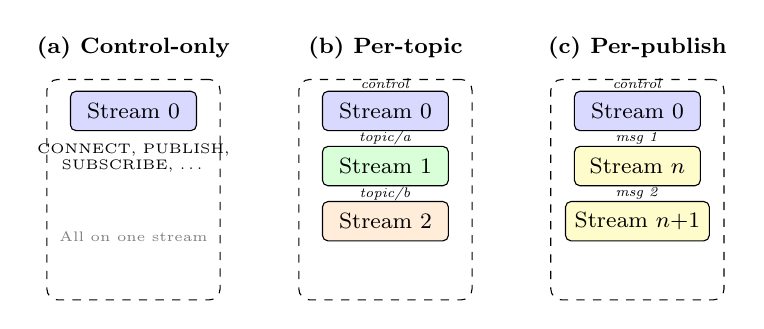
\begin{tikzpicture}[
    stream/.style={draw, rounded corners=2pt, minimum width=1.6cm, minimum height=0.5cm, font=\footnotesize},
    connbox/.style={draw, dashed, rounded corners=4pt, inner sep=6pt},
    label/.style={font=\footnotesize\bfseries},
    >=Stealth
]

\begin{scope}[shift={(0,0)}]
\node[label] at (0.8, 2.0) {(a) Control-only};
\node[connbox, minimum width=2.2cm, minimum height=2.8cm] at (0.8, 0.2) {};
\node[stream, fill=blue!15] at (0.8, 1.2) {Stream 0};
\node[font=\tiny, align=center] at (0.8, 0.6) {CONNECT, PUBLISH,\\SUBSCRIBE, \ldots};
\node[font=\tiny, text=gray] at (0.8, -0.4) {All on one stream};
\end{scope}

\begin{scope}[shift={(3.2,0)}]
\node[label] at (0.8, 2.0) {(b) Per-topic};
\node[connbox, minimum width=2.2cm, minimum height=2.8cm] at (0.8, 0.2) {};
\node[stream, fill=blue!15] at (0.8, 1.2) {Stream 0};
\node[stream, fill=green!15] at (0.8, 0.5) {Stream 1};
\node[stream, fill=orange!15] at (0.8, -0.2) {Stream 2};
\node[font=\tiny] at (0.8, 1.55) {\textit{control}};
\node[font=\tiny] at (0.8, 0.85) {\textit{topic/a}};
\node[font=\tiny] at (0.8, 0.15) {\textit{topic/b}};
\end{scope}

\begin{scope}[shift={(6.4,0)}]
\node[label] at (0.8, 2.0) {(c) Per-publish};
\node[connbox, minimum width=2.2cm, minimum height=2.8cm] at (0.8, 0.2) {};
\node[stream, fill=blue!15] at (0.8, 1.2) {Stream 0};
\node[stream, fill=yellow!20] at (0.8, 0.5) {Stream $n$};
\node[stream, fill=yellow!20] at (0.8, -0.2) {Stream $n$+1};
\node[font=\tiny] at (0.8, 1.55) {\textit{control}};
\node[font=\tiny] at (0.8, 0.85) {\textit{msg 1}};
\node[font=\tiny] at (0.8, 0.15) {\textit{msg 2}};
\end{scope}

\end{tikzpicture}
\caption{The three stream mapping strategies. (a)~Control-only multiplexes everything on stream~0. (b)~Per-topic assigns a dedicated stream per topic, providing topic-level isolation. (c)~Per-publish creates a new stream for each PUBLISH, providing message-level isolation.}
\label{fig:strategies}
\end{figure}

\textbf{Control-only} (Fig.~\ref{fig:strategies}a) uses a single bidirectional QUIC stream for all MQTT traffic. This is functionally equivalent to running MQTT over a single TCP connection and provides no HOL blocking mitigation. It serves as the QUIC baseline, isolating the effect of QUIC's transport mechanisms (encryption, congestion control) from stream multiplexing.

\textbf{Per-topic} (Fig.~\ref{fig:strategies}b) assigns each MQTT topic to a dedicated QUIC stream. Control packets (CONNECT, SUBSCRIBE, PINGREQ, etc.) use stream~0, while PUBLISH packets are routed to topic-specific streams. A hash map maintains the topic-to-stream mapping, creating streams lazily on first publish. This provides topic-level HOL blocking isolation: a retransmission delay on one topic's stream does not block delivery on other topics' streams.

\textbf{Per-publish} (Fig.~\ref{fig:strategies}c) creates a new unidirectional QUIC stream for each PUBLISH packet. This provides the finest-grained isolation---every message is independent---but at the highest overhead cost, as each message requires opening a new QUIC stream.

\subsection{Flow Header Protocol}

When using per-topic or per-publish strategies, the receiver must determine how to demultiplex incoming data on non-control streams. We introduce a lightweight \emph{flow header} prepended to the MQTT payload on data streams.

\begin{figure}
\centering
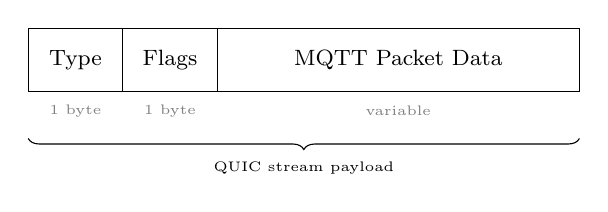
\begin{tikzpicture}[font=\footnotesize]
\draw (0,0) rectangle (7, 0.8);

\draw (1.2,0) -- (1.2,0.8);
\draw (2.4,0) -- (2.4,0.8);
\draw (7.0,0) -- (7.0,0.8);

\node at (0.6, 0.4) {Type};
\node at (1.8, 0.4) {Flags};
\node at (4.7, 0.4) {MQTT Packet Data};

\node[font=\tiny, text=gray] at (0.6, -0.25) {1 byte};
\node[font=\tiny, text=gray] at (1.8, -0.25) {1 byte};
\node[font=\tiny, text=gray] at (4.7, -0.25) {variable};

\draw[decorate, decoration={brace, amplitude=4pt, mirror}] (0, -0.6) -- (7, -0.6)
  node[midway, below=5pt, font=\tiny] {QUIC stream payload};
\end{tikzpicture}
\caption{Flow header format. The 2-byte header identifies the packet type and flags, enabling the receiver to parse data streams without full MQTT framing on stream~0.}
\label{fig:flow-header}
\end{figure}

The flow header (Fig.~\ref{fig:flow-header}) consists of two bytes: a type field identifying the MQTT packet type (PUBLISH for data streams) and a flags byte encoding QoS level, retain, and duplicate delivery (DUP) indicators. The receiver reads this header to determine how to parse the remainder of the stream. This is more efficient than transmitting the full MQTT fixed header on every stream, since the stream itself provides the framing boundary.

\subsection{Datagram Transport}

As an alternative to stream-based transport, \texttt{mqtt5} supports QUIC datagrams (RFC~9221) for QoS~0 messages. Datagrams bypass QUIC's stream layer entirely: messages are sent as unreliable frames within the QUIC connection, benefiting from QUIC's encryption and connection management but without reliability or ordering guarantees.

Datagram transport is designed for latency-sensitive telemetry where occasional message loss is acceptable. Since QUIC datagrams are subject to the connection's congestion window but not to per-stream flow control, lost messages are skipped rather than retransmitted. However, as both transports share the same per-connection congestion controller, the practical latency difference is small (see Section~\ref{sec:evaluation}).

\subsection{Broker Integration}

The client and broker configure their stream strategies independently. On the client side, the application selects a strategy (control-only, per-topic, or per-publish) before connecting; this governs how outbound PUBLISH packets are dispatched onto QUIC streams. On the broker side, a server-wide delivery strategy governs how the broker sends messages to subscribers. In a typical deployment, both sides are configured to the same strategy, but the architecture does not enforce this---a per-topic client can connect to a control-only broker, or vice versa.

For outbound delivery, the broker's stream manager maintains a per-connection topic-to-stream mapping. When configured for per-topic delivery, streams are created lazily on first use and reused for subsequent messages on the same topic, with LRU eviction to bound stream count. For per-publish delivery, the broker opens a new unidirectional stream for each message. On the receive side, the broker's QUIC acceptor classifies incoming streams by ID: stream~0 carries the full MQTT packet parser, while non-zero streams use the flow header parser to extract PUBLISH packets and route them into the topic distribution engine.

%% --- Implementation ---

\section{Implementation}
\label{sec:implementation}

\texttt{mqtt5}\footnote{\url{https://github.com/LabOverWire/mqtt-lib}} is an open-source MQTT library written in Rust. The library provides both a client and broker, supporting TCP, TLS~1.3, WebSocket, and QUIC transports. The QUIC implementation uses Quinn~\cite{quinn}, a Rust QUIC library built on the \texttt{tokio} async runtime.

\subsection{Transport Abstraction}

The library defines a \texttt{Transport} trait abstracting read/write operations over any underlying connection. For TCP and TLS, this wraps a single byte stream. For QUIC, the transport layer manages multiple streams through a \texttt{StreamDispatcher} that implements the configured strategy.

The stream dispatcher maintains a \texttt{HashMap<String, QuicStream>} for per-topic mapping, creating streams lazily on first use and reusing them for subsequent messages on the same topic. For per-publish, the dispatcher opens a new unidirectional stream for each PUBLISH and closes it after sending. Stream~0 (the initial bidirectional stream) is always reserved for control packets. Quinn's default behavior packs STREAM frames from multiple streams into single QUIC packets for efficiency. To isolate the effect of this frame packing on inter-stream coupling, we extended Quinn with a configurable frame packing policy: the default \emph{Greedy} policy preserves the original batching behavior, while a new \emph{StreamIsolated} policy restricts each packet to a single stream's data, preventing cross-stream coupling at the packet level.

\subsection{Connection Lifecycle}

QUIC connections follow the same MQTT session lifecycle as TCP connections. The CONNECT packet is always sent on stream~0. After CONNACK, subsequent PUBLISH packets are dispatched according to the client's configured stream strategy.

On the broker side, the QUIC acceptor spawns a dedicated task per connection. Incoming streams are classified by their stream ID: stream~0 receives the full MQTT packet parser, while non-zero streams use the flow header parser to extract PUBLISH packets and route them into the broker's topic distribution engine.

\subsection{Datagram Path}

When datagram mode is enabled, QoS~0 PUBLISH packets are sent as QUIC DATAGRAM frames. The MQTT packet is serialized with the flow header prepended and submitted via Quinn's \texttt{send\_datagram} API. The maximum datagram size is bounded by the connection's \texttt{max\_datagram\_size} parameter, which is negotiated during the QUIC handshake. Messages exceeding this limit fall back to stream transport.

On the receive path, datagrams are delivered via a separate channel from stream data. The broker's QUIC handler polls both the stream accept loop and the datagram receive loop concurrently, feeding both into the same message processing pipeline.

\subsection{Benchmarking Infrastructure}

The library includes an integrated benchmarking tool (\texttt{mqttv5 bench}) that measures latency and throughput. Latency mode embeds microsecond timestamps in payloads and computes p50/p95/p99 percentiles. Throughput mode counts messages per second over a configurable duration with warmup. Both modes support configurable publisher/subscriber counts, QoS levels, payload sizes, and transport parameters.

Network impairment is applied externally via \texttt{tc-netem}, and broker/client resource usage (RSS, CPU, network I/O) is sampled at 1\,Hz during each run using procfs monitors.

%% --- Evaluation ---

\section{Evaluation}
\label{sec:evaluation}

We evaluate \texttt{mqtt5} across five experiments measuring connection establishment, head-of-line blocking, throughput, stream strategy behavior, and datagram transport. All experiments use QoS~0 unless otherwise noted.

\subsection{Experimental Setup}

\begin{table}
\centering
\caption{Experimental parameters across all five experiments.}
\label{tab:params}
\begin{tabular}{ll}
\toprule
Parameter & Value \\
\midrule
Hardware & GCP n2-standard-4 (4 vCPU, 16 GB RAM) \\
Topology & Co-located pub/sub (Exp 2), separate VMs (others) \\
Region & us-west1-b (same zone, $<$1ms baseline RTT) \\
OS & Debian 12, kernel 6.1 \\
Network emulation & \texttt{tc-netem} on broker (symmetric) \\
QUIC implementation & Quinn 0.11 (Rust) \\
TLS & rustls 0.23 (TLS 1.3 only) \\
Congestion control & QUIC: NewReno / TCP: CUBIC \\
Payload size & 256 bytes (all experiments) \\
Publish rate & 500 msg/s fixed (Exp 2), max throughput (others) \\
Measurement & 60s duration, 5s warmup (30s/0s warmup for Exp 1) \\
Runs per config & 15 (all experiments) \\
Frame packing & Greedy (default); StreamIsolated (Exp 2 ablation) \\
\bottomrule
\end{tabular}
\end{table}

Table~\ref{tab:params} summarizes the common parameters. Network impairment is applied symmetrically on the broker interface using \texttt{tc-netem}. Each experiment varies one or two factors while holding others constant. Experiment~2 uses co-located publisher and subscriber on a single client VM to eliminate network variability between pub/sub; all other experiments use separate VMs.

\subsection{Experiment 1: Connection Establishment Latency}

We measure cold-start connection latency across TCP, TLS~1.3, and QUIC at five one-way delays (0, 25, 50, 100, 200\,ms) using 100 sequential connections per run.

\begin{figure}
\centering
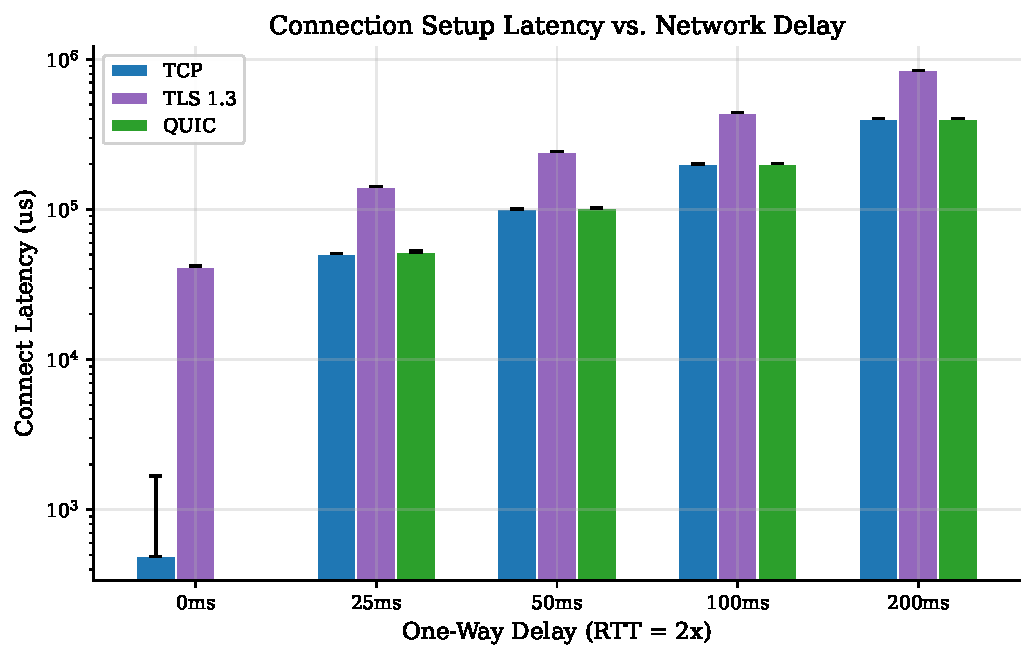
\includegraphics[width=\columnwidth]{Figure_4}
\caption{Connection latency (p50 bars, p95 whiskers) across network delays. QUIC's integrated TLS handshake achieves comparable latency to raw TCP despite cryptographic overhead, and outperforms the separate TCP+TLS~1.3 handshake at all RTTs.}
\label{fig:conn-latency}
\end{figure}

Fig.~\ref{fig:conn-latency} shows that QUIC 1-RTT connection establishment matches TCP's cold-connect latency at all tested delays. TLS~1.3 over TCP consistently adds one additional round trip. At 200\,ms delay, QUIC connects in 402\,ms (p50) versus TCP's 400\,ms and TLS's 842\,ms. The integrated handshake eliminates the sequential TCP+TLS penalty without sacrificing security. We did not test QUIC 0-RTT resumption, which could further reduce connection latency for returning clients.

\subsection{Experiment 2: Head-of-Line Blocking}

This experiment is the core motivation for MQTT-over-QUIC multistream transport. We publish to 8 topics simultaneously at a fixed rate of 500\,msg/s and measure whether latency fluctuations on one topic propagate to others. The fixed rate is chosen to remain well below connection capacity at all loss rates (the minimum sustained capacity under 5\% loss at 25\,ms RTT exceeds 500\,msg/s), ensuring that any observed latency variation reflects transport-layer behavior rather than queue buildup from rate saturation.

We quantify HOL blocking using two complementary metrics. \emph{Inter-topic spread} measures the maximum difference between per-topic mean latencies within 100\,ms time windows: high spread means topics experience different latencies (isolation), while low spread means topics are coupled. \emph{Spike isolation ratio} measures the fraction of latency spikes that co-occur across all topics: a ratio of 1.0 means every spike affects all topics simultaneously (full HOL blocking), while lower values indicate independent spikes.

\begin{figure}
\centering
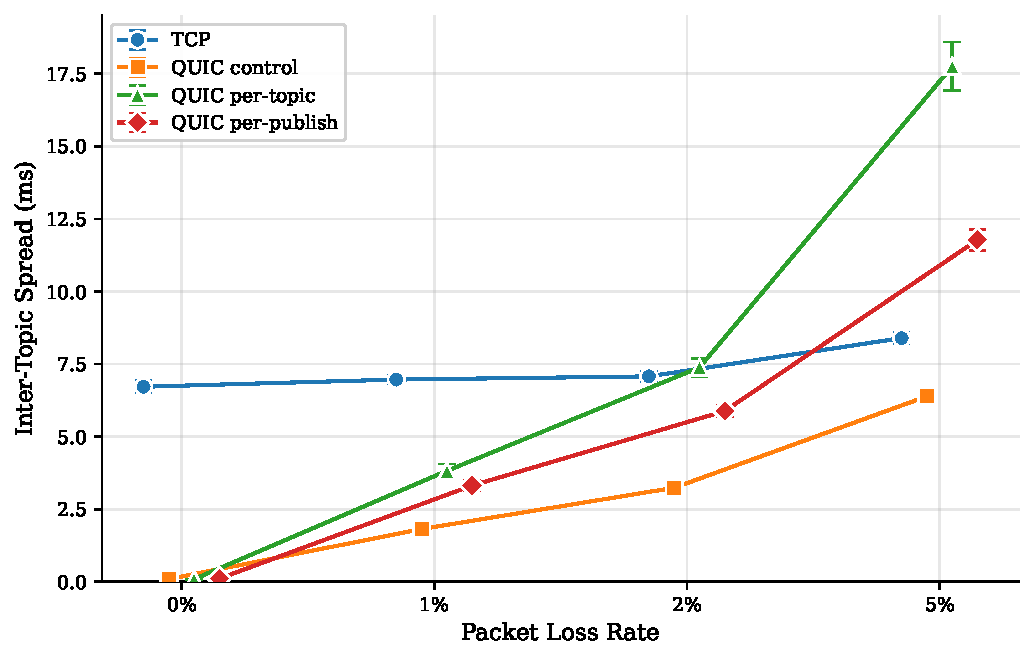
\includegraphics[width=\columnwidth]{Figure_1}
\caption{Inter-topic latency spread across packet loss rates (25\,ms RTT, 8 topics, 15 runs per configuration). Per-topic QUIC spread amplifies 200$\times$ from baseline to 5\% loss, consistent with independent per-stream loss recovery. TCP spread increases only 1.2$\times$, indicating that all topics remain tightly coupled under loss.}
\label{fig:spread}
\end{figure}

Fig.~\ref{fig:spread} shows inter-topic spread at 25\,ms RTT across four loss rates with 15 runs per configuration. At 0\% loss, all transports show low spread: TCP at 6.7\,ms, QUIC per-topic at 0.09\,ms, per-publish at 0.11\,ms, and control-only at 0.09\,ms. Under 5\% loss, per-topic QUIC spread amplifies to 17.8\,ms (200$\times$ baseline), while TCP increases to only 8.4\,ms (1.2$\times$). Per-publish shows 107$\times$ amplification and control-only shows 71$\times$.

The high spread for multi-stream QUIC strategies under loss is consistent with QUIC's independent per-stream loss recovery~\cite{rfc9000}: when a packet carrying data for one topic is lost, only that topic's stream should experience retransmission delay, while other streams continue unaffected. TCP's single byte stream provides no such isolation, which is consistent with the low spread amplification observed. In absolute terms, TCP's coupled degradation is also more severe: at 5\% loss, TCP p95 latency reaches 180\,ms and p99 reaches 355\,ms across all topics uniformly, while QUIC per-topic achieves 99\,ms p95 and 183\,ms p99 with the impact confined to individually affected streams.

\begin{figure}
\centering
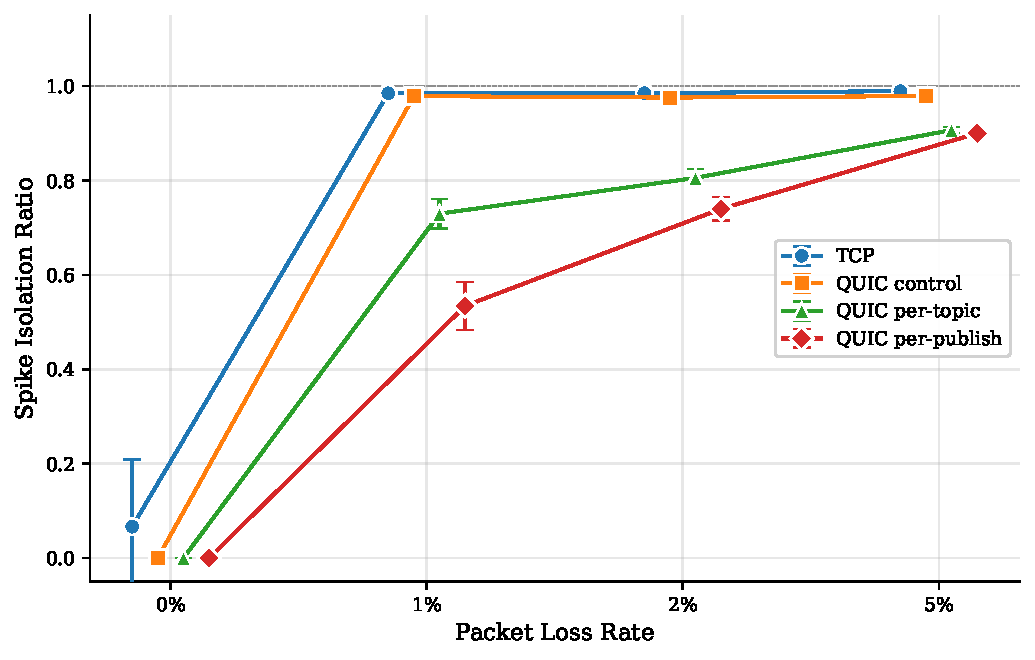
\includegraphics[width=\columnwidth]{Figure_2}
\caption{Spike isolation ratio across packet loss rates. A ratio of 1.0 means all latency spikes co-occur across topics (full HOL blocking). TCP remains near 1.0 at all loss rates, while per-topic (0.73) and per-publish (0.53) QUIC show progressively more independent spike behavior at 1\% loss.}
\label{fig:spike-iso}
\end{figure}

Fig.~\ref{fig:spike-iso} provides a complementary view through spike isolation ratio. TCP maintains a ratio near 1.0 at all loss rates (0.98 at 1\% loss), confirming that virtually all latency spikes propagate to every topic. Per-topic QUIC drops to 0.73 and per-publish to 0.53 at 1\% loss, indicating that 27--47\% of spikes affect individual topics independently. Control-only QUIC remains at 0.98, consistent with its single-stream architecture that provides no inter-topic isolation.

QUIC's congestion control operates per-connection~\cite{rfc9002, rfc9308}, sharing a single congestion window across all streams. We hypothesize that this shared congestion response limits the degree of isolation: a loss event reduces the congestion window for all concurrent streams, even though stream-level loss recovery is independent. This is consistent with per-topic isolation being partial (0.73) rather than complete ($\approx$0).

\textbf{Ablation: frame packing policy.} To determine whether the partial correlation observed at 0\% loss reflects QUIC's congestion control architecture or an implementation-level artifact, we conducted a control experiment varying Quinn's frame packing behavior. By default, Quinn packs STREAM frames from multiple streams into single QUIC packets---a hardcoded optimization we term \emph{Greedy} packing. When a single packet is lost, all streams whose data it carried experience retransmission delay simultaneously, potentially creating artificial inter-stream coupling. We extended Quinn with a \emph{StreamIsolated} policy that restricts each packet to a single stream's data, eliminating this cross-stream coupling at the packet level. We tested both policies using the same parameters as the main experiment (500\,msg/s, 8 topics, 25\,ms RTT, 15 runs per configuration).

At 0\% loss, the baseline correlation persists under StreamIsolated packing: per-topic windowed correlation is 0.64 versus 0.55 with Greedy. Without packet loss, no retransmissions occur, so packet-level frame co-location cannot be the cause. QUIC specifies a single congestion controller per connection~\cite{rfc9002}, and all streams share a single UDP socket. We hypothesize that this shared per-connection state---pacer, congestion window, and socket---creates correlated jitter across streams regardless of how frames are packed into packets. Under loss, however, StreamIsolated per-topic packing shows 26\% higher inter-topic spread (22.5\,ms versus 17.8\,ms at 5\% loss) and 6\% lower spike isolation ratio (0.85 versus 0.91 at 5\% loss), demonstrating genuine per-stream isolation improvement when retransmission events cannot cross stream boundaries within a single packet (Fig.~\ref{fig:frame-packing}).

The effect is asymmetric across strategies. For per-publish, StreamIsolated packing is counterproductive: p50 latency at 5\% loss rises from 29\,ms to 111\,ms. We hypothesize that isolated packing creates more QUIC packets for ephemeral streams (each publish opens and closes a new stream), increasing the volume subject to loss and retransmission, which may overwhelm connection capacity under high loss. This interaction between frame packing policy and stream lifetime---beneficial for persistent streams, harmful for ephemeral ones---has implications for adaptive transport configuration (Section~\ref{sec:discussion}).

\begin{figure}
\centering
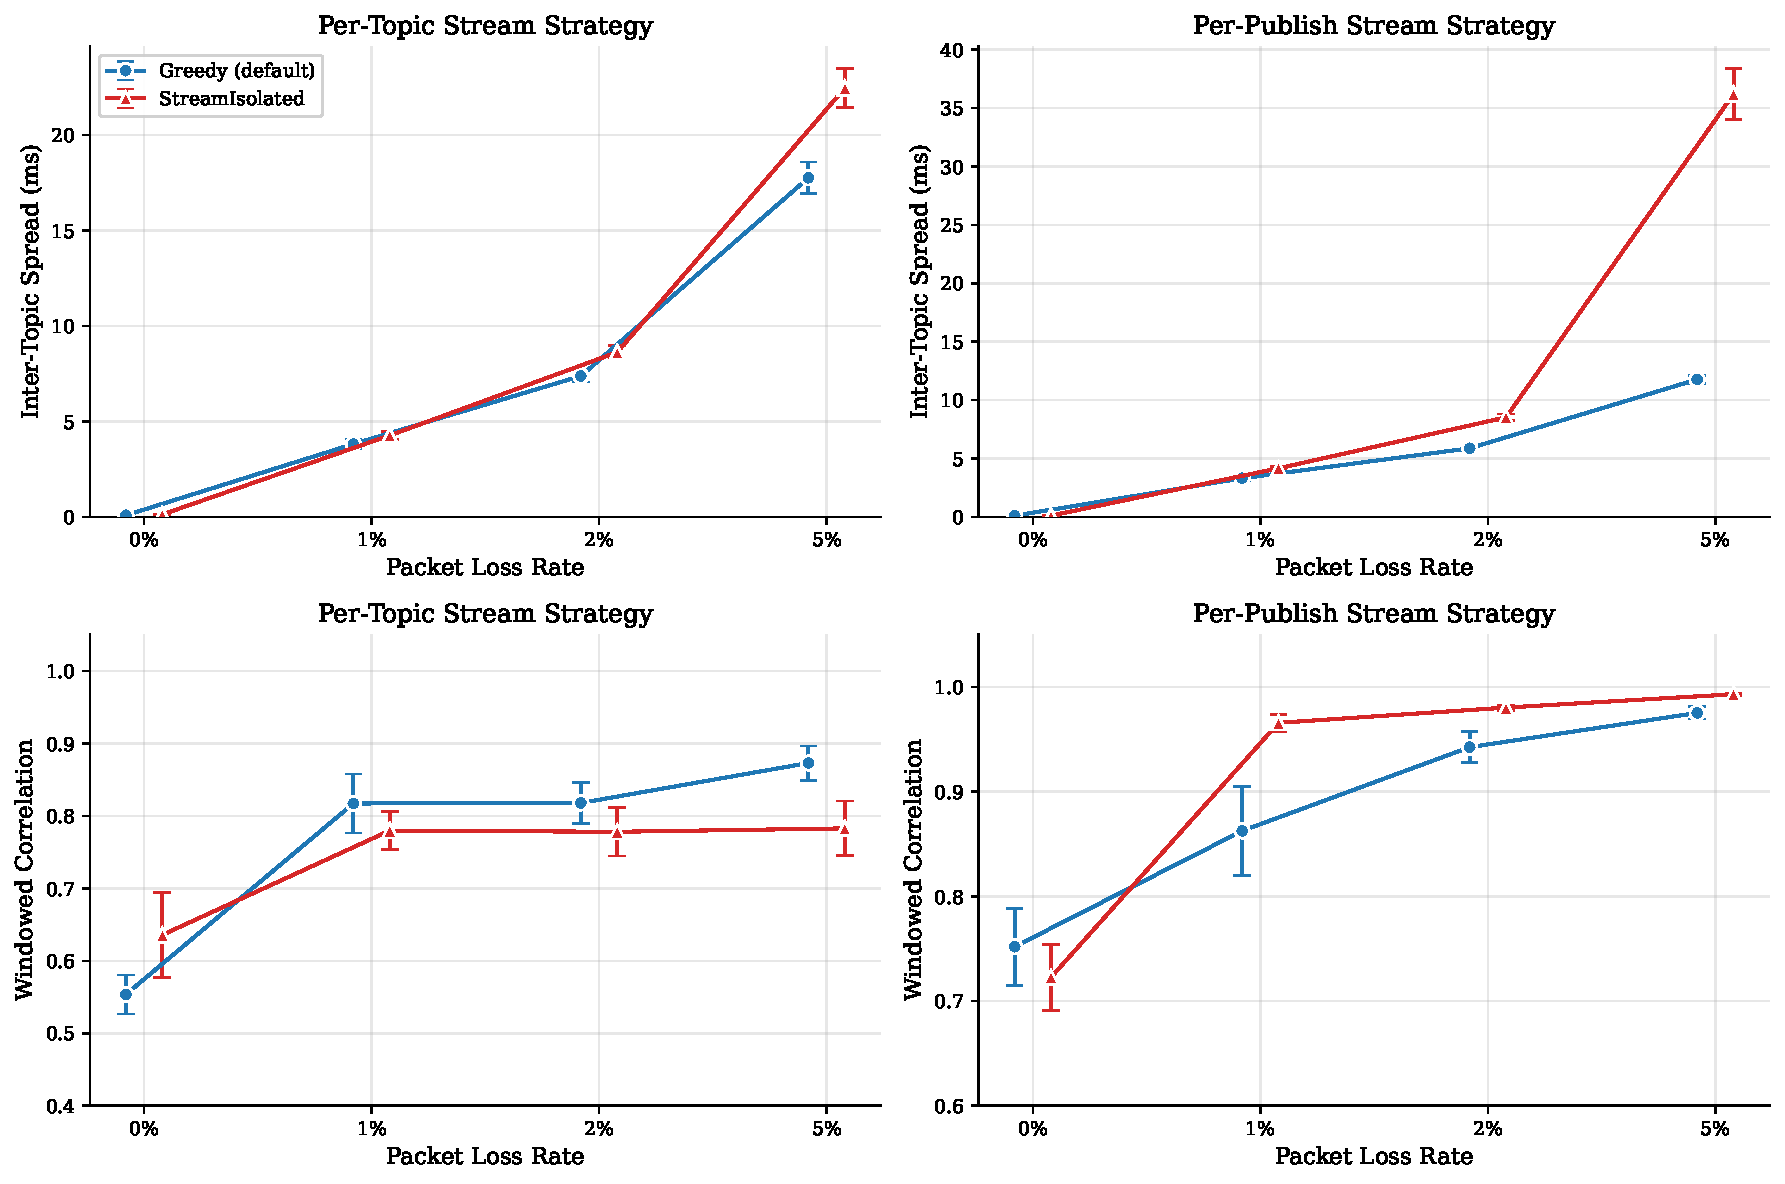
\includegraphics[width=\columnwidth]{Figure_8}
\caption{Effect of frame packing policy on HOL blocking metrics. \emph{Greedy} packing (default) batches multiple streams per packet; \emph{StreamIsolated} restricts each packet to one stream. For per-topic (left), StreamIsolated improves spread and reduces correlation under loss. For per-publish (right), StreamIsolated increases overhead, degrading performance at high loss rates.}
\label{fig:frame-packing}
\end{figure}

\begin{figure}
\centering
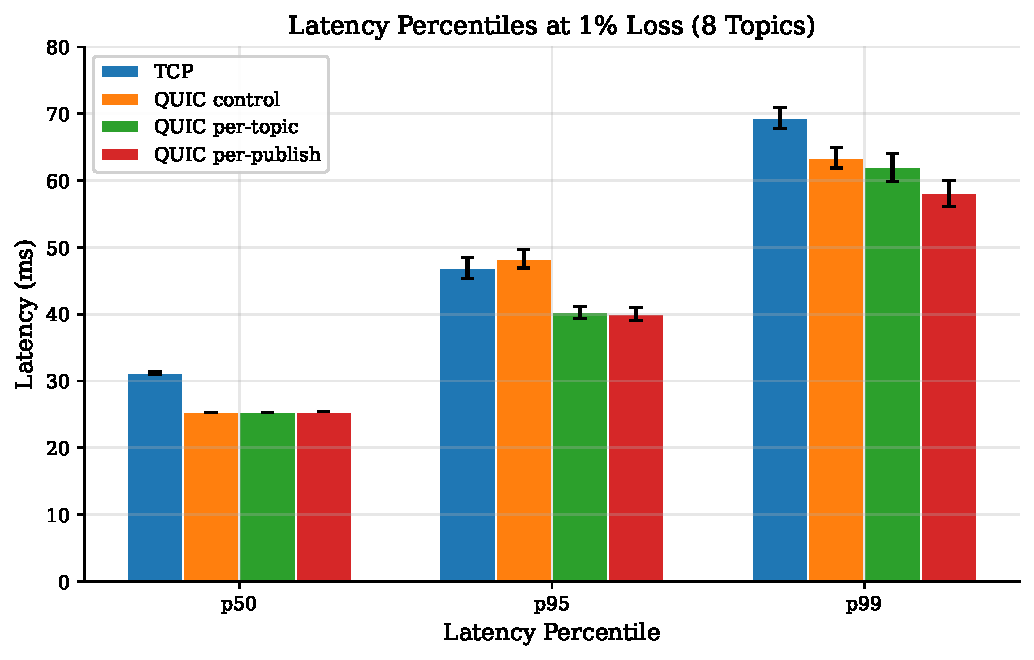
\includegraphics[width=\columnwidth]{Figure_3}
\caption{Latency percentiles at 1\% loss, 25\,ms RTT. TCP exhibits higher tail latency than all QUIC strategies, with the gap widening at higher percentiles. Multi-stream QUIC strategies (per-topic, per-publish) achieve the lowest p95 and p99 values.}
\label{fig:lat-percentiles}
\end{figure}

Fig.~\ref{fig:lat-percentiles} shows latency percentiles at 1\% loss. TCP exhibits the highest tail latency across all percentiles, with the gap between TCP and QUIC widening from p50 to p99. Multi-stream QUIC strategies (per-topic, per-publish) achieve the lowest p95 and p99 values, consistent with independent per-stream loss recovery reducing tail latency when retransmission delays are confined to individual streams rather than stalling the entire connection.

\subsection{Experiment 3: Throughput Under Loss}

We measure sustained throughput using 4 publishers and 4 subscribers at 10\,ms one-way delay across loss rates from 0\% to 10\%.

\begin{figure}
\centering
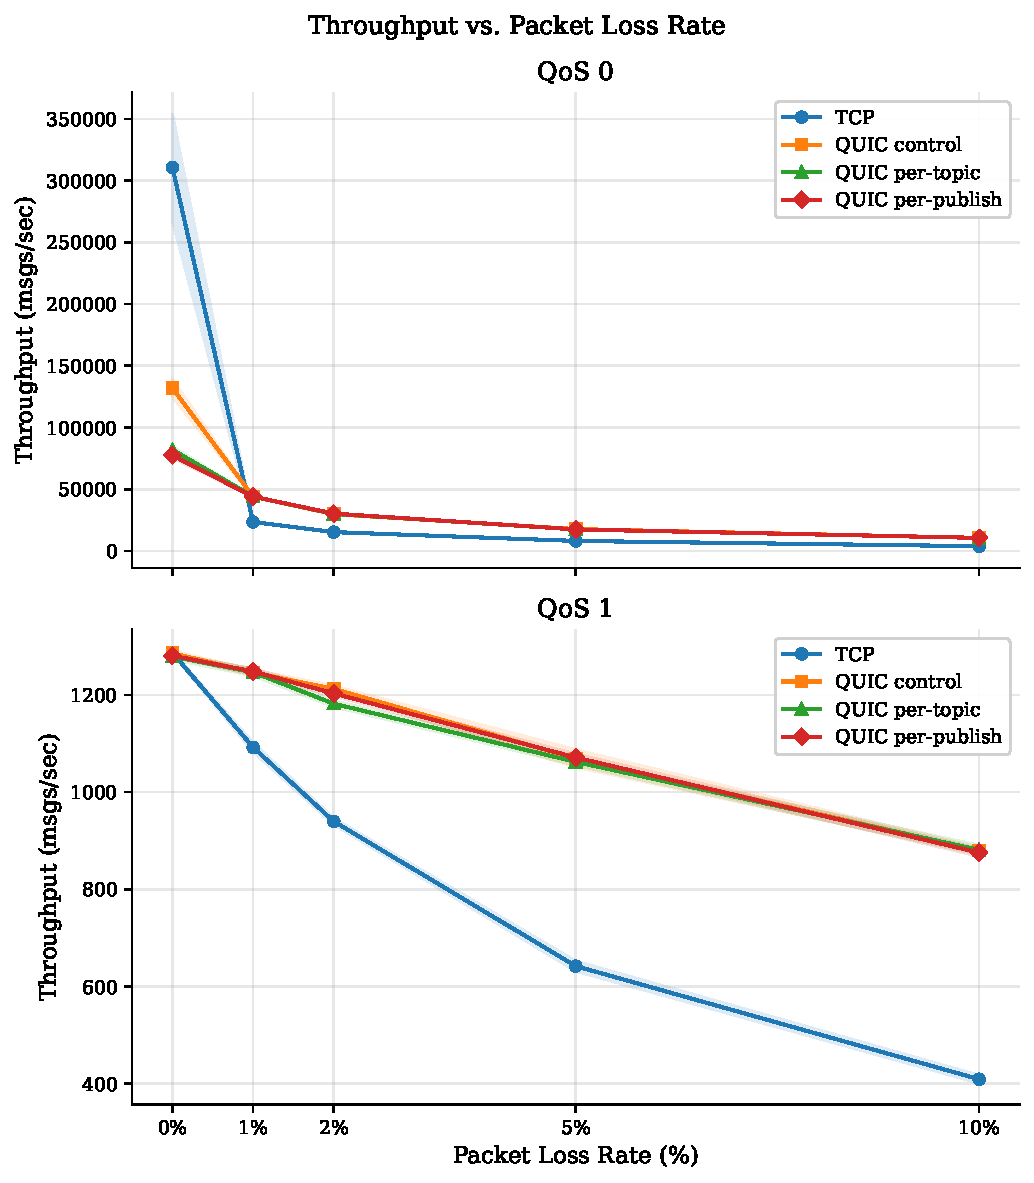
\includegraphics[width=\columnwidth]{Figure_5}
\caption{Throughput vs.\ packet loss for QoS~0 (top) and QoS~1 (bottom). TCP outperforms all QUIC strategies at baseline (0\% loss), but under loss ($\geq$1\%) all QUIC strategies outperform TCP.}
\label{fig:throughput-loss}
\end{figure}

Fig.~\ref{fig:throughput-loss} reveals that at 0\% loss, TCP outperforms all QUIC strategies in raw throughput. With QoS~0, TCP achieves 311K\,msg/s versus QUIC control-only at 132K\,msg/s, per-topic at 82K\,msg/s, and per-publish at 77K\,msg/s. The throughput gap at baseline is consistent with QUIC's additional per-packet processing overhead, though we did not isolate individual contributing factors (see Section~\ref{sec:discussion} for further analysis).

Under loss ($\geq$1\%), the ordering reverses: all QUIC strategies outperform TCP, achieving 1.9$\times$ TCP's throughput at 1\% loss and 2.8$\times$ at 10\% loss. Per-publish QUIC matches control-only throughput under loss, suggesting that stream creation overhead becomes negligible relative to loss recovery delays.

QoS~1 throughput drops to approximately 1.3K\,msg/s across all transports at 0\% loss, as the per-message acknowledgment round-trip dominates. Under loss, QUIC maintains higher QoS~1 throughput than TCP (880 versus 409\,msg/s at 10\% loss).

\subsection{Experiment 4: Stream Strategy Comparison}

We compare the three stream mapping strategies (control-only, per-publish, per-topic) while varying topic count (1, 4, 8, 16) at 25\,ms one-way delay and 2\% packet loss to understand how strategy selection interacts with workload structure under representative IoT conditions.

\begin{figure}
\centering
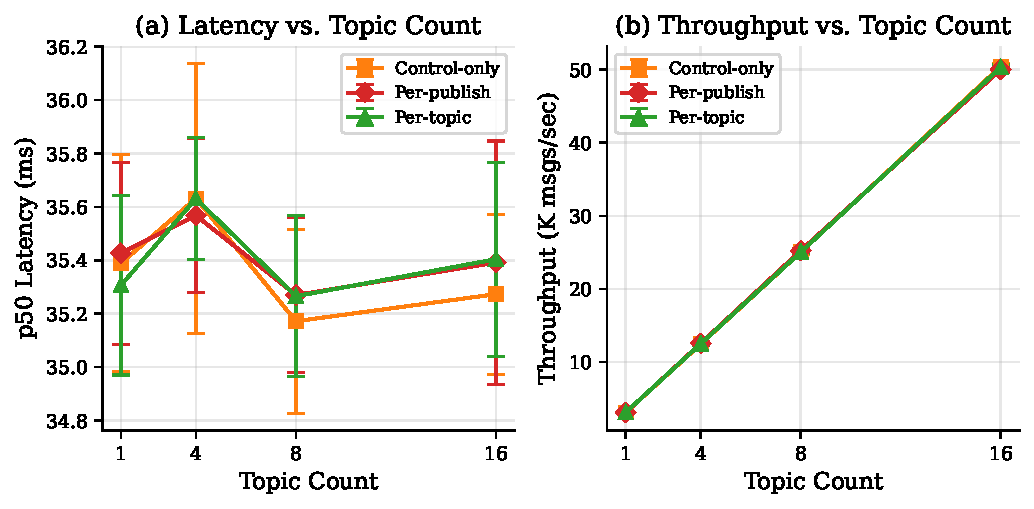
\includegraphics[width=\columnwidth]{Figure_7}
\caption{Strategy comparison across topic counts. (a)~Latency is stable across all strategies and topic counts. (b)~Throughput scales linearly with topic count for all strategies.}
\label{fig:strategy-comparison}
\end{figure}

Fig.~\ref{fig:strategy-comparison} shows that latency is stable at approximately 35\,ms across all strategies and topic counts, indicating that stream management overhead does not materially affect per-message latency in this workload. Throughput scales linearly with topic count for all strategies. At 16 topics, all three strategies converge to approximately 50K\,msg/s with no measurable throughput difference between them, indicating that stream management overhead is negligible at this workload scale.

\subsection{Experiment 5: Datagram vs.\ Stream Transport}

QUIC datagrams (RFC~9221) bypass the stream abstraction entirely, sending messages as unreliable datagrams within the QUIC connection. We compare datagram transport against stream-based transport at 50\,ms delay across four loss rates.

\begin{figure}
\centering
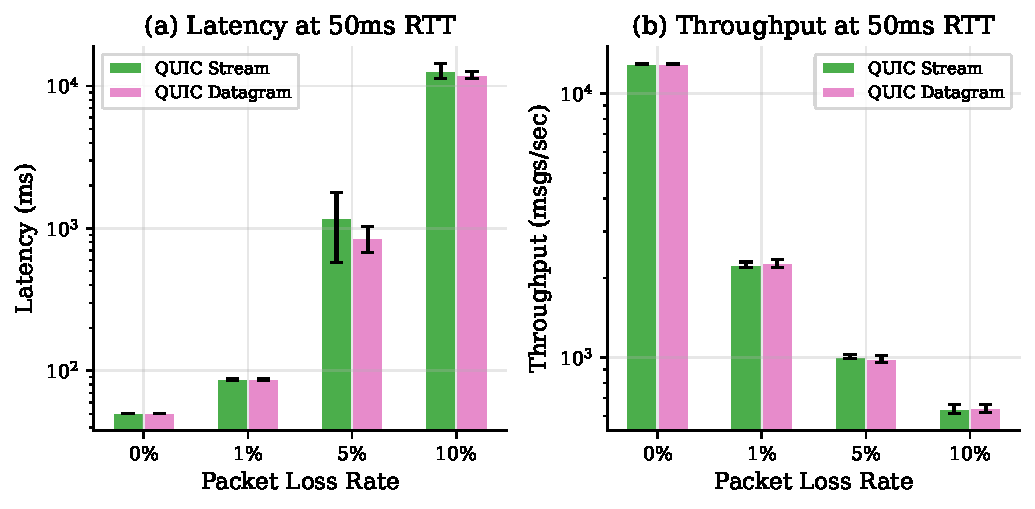
\includegraphics[width=\columnwidth]{Figure_6}
\caption{Datagram vs.\ stream transport at 50\,ms RTT. (a)~Latency distributions overlap at all loss rates, with high run-to-run variance under loss. (b)~Throughput is comparable since both transports share the same QUIC connection and congestion controller.}
\label{fig:datagram}
\end{figure}

Fig.~\ref{fig:datagram} shows that at 50\,ms RTT, datagram and stream transport are statistically indistinguishable at all loss rates. At 0\% loss, both achieve 12.9K\,msg/s throughput and 50.3\,ms p50 latency. Under loss, both transports degrade similarly: at 5\% loss, stream p50 is 1,188$\pm$1,070\,ms and datagram p50 is 854$\pm$308\,ms---the stream distribution's high variance (90\% coefficient of variation) means these values overlap within error bars. At 10\% loss, both exhibit multi-second latencies (stream 12.9$\pm$2.7\,s, datagram 12.0$\pm$1.3\,s). Throughput is comparable at all conditions ($\approx$1,000\,msg/s at 5\% loss), as both share the same QUIC connection and congestion controller. The theoretical advantage of datagrams---skipping retransmission of lost messages---is not observed in our measurements, possibly because both transports share the same per-connection congestion controller~\cite{rfc9002}.

%% --- Discussion ---

\section{Discussion}
\label{sec:discussion}

\subsection{Strategy Selection Guidelines}

Our results suggest the following guidelines for practitioners selecting a stream mapping strategy:

\textbf{Use control-only} when throughput is the primary concern and topics are not independent. This strategy adds QUIC's security benefits (integrated TLS~1.3) and connection management (migration, 0-RTT potential) with minimal overhead compared to TCP. It provides no inter-topic isolation (spike isolation ratio 0.98, comparable to TCP's 0.98), making it appropriate for single-topic workloads or scenarios where HOL blocking is acceptable.

\textbf{Use per-topic} when topic independence matters and the number of topics is bounded. At 1\% loss---representative of typical wireless IoT conditions---per-topic mapping already provides measurable isolation: inter-topic spread amplifies 42$\times$ from baseline, and 27\% of latency spikes affect individual topics independently (spike isolation ratio 0.73 versus TCP's 0.98). At higher loss (5\%), spread amplification reaches 200$\times$. Per-topic throughput is 62\% of control-only at baseline. The overhead scales with the number of active topics, not the message rate, making it efficient for workloads with moderate topic counts (tens to hundreds). StreamIsolated frame packing further improves isolation (+26\% spread, $-$6\% spike ratio at 5\% loss) with modest latency cost, making it recommended for loss-prone deployments. This is the recommended default for multi-topic IoT deployments on lossy networks.

\textbf{Use per-publish} only when message-level isolation is required and throughput is secondary. Per-publish shows the strongest spike isolation (ratio 0.53 at 1\% loss, meaning 47\% of spikes are topic-independent), but the per-message stream creation overhead makes this strategy unsuitable for high-throughput workloads. StreamIsolated frame packing should be avoided for this strategy, as our measurements show significant latency degradation under loss (p50 rises from 29\,ms to 111\,ms at 5\% loss). It may be appropriate for low-rate command-and-control channels where every message must be independently deliverable.

\textbf{Use datagrams} for latency-sensitive telemetry with QoS~0 where occasional message loss is acceptable. At 50\,ms RTT, datagrams show no statistically significant latency or throughput advantage over streams. Datagrams remain a valid design choice for applications that explicitly tolerate message loss, but our results do not demonstrate a measurable performance benefit at representative IoT RTTs. They are unsuitable for QoS~1 or QoS~2 workloads that require acknowledgment semantics.

\subsection{Throughput--Isolation Tradeoff}

At baseline (0\% loss), unencrypted TCP achieves 2.4--4.0$\times$ the throughput of QUIC strategies (Experiment~3). This comparison is inherently asymmetric: QUIC mandates encryption, while our TCP baseline operates without TLS. A fairer throughput comparison would use TCP with TLS~1.3, which would narrow the gap by adding comparable per-packet encryption overhead to TCP. However, the absolute throughput difference at 0\% loss is less important than the practical picture: in real IoT deployments, packet loss is the norm rather than the exception, and QUIC already outperforms even unencrypted TCP at just 1\% loss (1.9$\times$), reaching 2.8$\times$ at 10\% loss. The implication is that QUIC provides a net advantage in realistic conditions: it delivers higher throughput under loss, provides stream-level isolation for independent topic flows, and includes encryption by default---eliminating the need for a separate TLS layer.

\subsection{HOL Blocking Isolation: Partial but Meaningful}

Our HOL blocking results show that QUIC stream multiplexing provides \emph{partial} rather than \emph{complete} isolation between topics. The spike isolation ratio for per-topic QUIC drops to 0.73 at 1\% loss rather than approaching 0 (full independence). QUIC's congestion control operates per-connection~\cite{rfc9002}: a loss event reduces the congestion window for all concurrent streams, even though stream-level loss recovery is independent. We hypothesize that this shared congestion response is responsible for the partial isolation. The inter-topic spread metric is consistent with this interpretation---topics experience different retransmission delays (high spread) but partially correlated congestion responses (spike co-occurrence).

We tested whether Quinn's default frame packing---batching STREAM frames from multiple streams into single QUIC packets---contributes to this baseline correlation by running the same experiment with StreamIsolated packing, which restricts each packet to a single stream's data. The correlation persists (0.64 versus 0.55 at 0\% loss), confirming that it is not caused by frame co-location. Without packet loss, no retransmissions occur, so frame co-location has no effect; all streams still share a single congestion controller, pacer, and UDP socket~\cite{rfc9002}, which we hypothesize creates correlated jitter independent of frame packing. Under loss, however, StreamIsolated measurably improves per-topic isolation at 5\% loss, with 26\% higher inter-topic spread and a 6\% lower spike isolation ratio---both consistent with reduced cross-stream coupling at the packet level. However, for per-publish, isolated packing is counterproductive: p50 latency rises from 29\,ms to 111\,ms at 5\% loss with StreamIsolated versus Greedy, possibly because the increased packet count from ephemeral streams amplifies retransmission overhead.

\subsection{Future Work}

Several directions emerge from this work. First, evaluating 0-RTT connection resumption would quantify the benefit for mobile clients that reconnect frequently. Second, testing connection migration could demonstrate QUIC's advantage for devices that change network interfaces. Third, exploring adaptive strategy selection---where the broker dynamically switches strategies based on observed network conditions---could automate the throughput--isolation tradeoff. Additionally, exploring adaptive frame packing that automatically selects Greedy packing for per-publish and StreamIsolated for per-topic based on the negotiated stream strategy could optimize the transport layer without manual configuration. Finally, extending the evaluation to constrained devices (e.g., ESP32, Raspberry Pi) would assess whether QUIC's computational overhead is viable for resource-limited IoT endpoints.

%% --- Conclusion ---

\section{Conclusion}
\label{sec:conclusion}

We presented three configurable stream mapping strategies for running MQTT over QUIC. Through five experiments on controlled infrastructure, we demonstrated that per-topic QUIC stream mapping provides measurable HOL blocking isolation: inter-topic latency spread amplifies 200$\times$ under 5\% packet loss, consistent with independent stream loss recovery allowing topics to experience different retransmission delays rather than stalling together as TCP does (1.2$\times$ spread amplification). Spike isolation ratio corroborates this---at 1\% loss, 27\% of per-topic QUIC latency spikes affect individual topics independently, versus less than 2\% for TCP. The isolation is partial rather than complete, which we attribute to QUIC's per-connection congestion control that shares a single congestion window across all streams.

Our evaluation reveals a nuanced throughput tradeoff: at baseline (0\% loss), TCP achieves 2.4--4.0$\times$ the throughput of QUIC strategies depending on workload, but under loss ($\geq$1\%) QUIC outperforms TCP by up to 2.8$\times$. Per-topic mapping achieves 62\% of single-stream QUIC throughput at baseline. QUIC datagrams show no statistically significant performance difference from streams at representative IoT RTTs.

These results provide practitioners with concrete guidance for deploying MQTT over QUIC in IoT systems: use per-topic mapping for multi-topic workloads on lossy networks where independent stream recovery provides meaningful isolation and QUIC's throughput advantage under loss is beneficial, and use TCP when baseline throughput on reliable networks is the dominant concern. The implementation is available as open-source software.

\section*{Declaration of Generative AI and AI-Assisted Technologies in the Manuscript Preparation Process}

During the preparation of this work the author used Claude (Anthropic) in order to assist with manuscript drafting, data analysis scripting, and editing. After using this tool, the author reviewed and edited the content as needed and takes full responsibility for the content of the published article.

\section*{Data Availability}

The experimental data and analysis scripts used in this study are available in the project repository at \url{https://github.com/LabOverWire/mqtt-lib}.

\printcredits

\bibliographystyle{cas-model2-names}
\bibliography{references}

\end{document}
